\chapter{Introducción}

\section{Justificación}
Las aplicaciones y páginas web que se dedican a la predicción del tiempo meteorológico en nuestro país utilizan mayoritariamente los datos que aportan los satélites geoestacionarios METEOSAT, observatorios meteorológicos, radares y multitud de equipo diferente distribuido por toda la península que envían datos a la Agencia Estatal de Meteorología de España o AEMET.

Estos datos recogidos se han vuelto más precisos a lo largo de los años gracias al desarrollo de la tecnología y, por tanto, hemos conseguido cada vez mejores predicciones meteorológicas \cite{intro_1}. No solo se ha mejorado la precisión de los datos recogidos, sino que también se consigue tener más información con un acceso mucho más rápido y cómodo.

Históricamente, las distintas estaciones o centros de mediciones meteorológicos requerían de una constante supervisión e intervención humana para funcionar. Sin embargo, hoy disponemos de estaciones automatizadas que pueden aportar datos de forma continua, dejando la intervención humana solo para sus mantenimientos correspondientes \cite{intro_2}.

Este desarrollo de la tecnología respecto al mundo de la meteorología es más importante de lo que muchas personas puedan concebir. Nuestra vida siempre se ha visto atada de una manera u otra a los cambios en el tiempo. Gracias a las predicciones, agricultores, ganaderos y pescadores entre otros trabajos han podido llevar de una manera óptima su labor, preparándose y actuando en función del tiempo. Para el resto de personas que no estamos relacionados con esos ámbitos también nos afecta, aunque sea en menor medida, si sabemos con anterioridad los cambios en las temperaturas podremos vestirnos de una manera u otra antes de salir, por ejemplo. Por eso es tan importante la meteorología, nuestra vida o aspectos de ella giran en torno al tiempo atmosférico.

Y, aún así, seguimos sin tener predicciones perfectas. Como he comentado, la tecnología ha avanzado mucho estos últimos años y ha mejorado las predicciones, ¿por qué siguen sin ser perfectas? ¿Por qué sigue habiendo fallos? ¿Incluso por qué veo que dos aplicaciones me dan información diferente sobre una misma localidad?

Estos problemas suelen estar relacionados con dos situaciones: los centros de recogida de datos no se encuentran en la localidad como tal o se sitúan en otra próxima, ocurre sobre todo en pueblos muy pequeños; dos aplicaciones pueden tener la misma fuente de datos, pero sus métodos de predicción son distintos por lo que varían \cite{intro_3}.

\section{Objetivos}

Con todo lo anterior en mente, el objetivo principal del proyecto consiste en obtener y mantener un confort térmico en la smarthome de la UAL óptimo. Para ello se requerirán de algunos objetivos más pequeños:

\begin{itemize}
    \item Obtener datos atmosféricos a partir de los sensores instalados y guardarlos en bases de datos.
    \begin{itemize}
        \item Estudio de los sensores instalados actualmente.
        \item Acceso a los sensores a través de la API de la smarthome.
        \item Script en Python que acceda automáticamente a la API y registre los datos.
        \item Instalación y preparación de bases de datos.
    \end{itemize}
    \item Utilizar los datos obtenidos para representarlos visualmente y obtener el nivel de confort.
    \begin{itemize}
        \item Utilizar los datos guardados en las bases de datos para representarlos en una interfaz con gráficas y otros indicadores.
        \item Investigar y utilizar un modelo para obtener el confort de la smarthome.
    \end{itemize}
    \item Actuar sobre los dispositivos de la casa con el objetivo de mantener o modificar el grado de confort calculado.
    \begin{itemize}
        \item Script en Python que toma decisiones en función del confort térmico actual y actúe sobre los dispositivos de la casa.
        \item Informar al usuario de la casa a través del altavoz Sonos el estado actual del confort y las acciones tomadas para modificarlo.
    \end{itemize}
\end{itemize}

\section{SmartHome y KNX}

La \textit{smarthome} de la Universidad de Almería es un laboratorio construido con el objetivo de que tanto personal universitario como los propios alumnos pudieran investigar, trabajar y aprender sobre \textit{IoT}. La estancia está totalmente conectada a través del protocolo KNX, con el que se ha construido un ecosistema de dispositivos, sensores y actuadores con los que continuamente se realizan avances y nuevas investigaciones.

Algunos de los sensores que la componen son de temperatura, humedad, CO2 o luminosidad. Además de actuadores como los estores de las ventanas, aire acondicionado o incluso las luces. Sin embargo, no todo está conectado por KNX, sino que hay otros dispositivos conectados a la subred de la smarthome a través de TCP/HTTP por WiFi, como el altavoz Sonos, cámaras de seguridad o la Smart TV \cite{intro_4}.

\begin{figure}
    \centering
    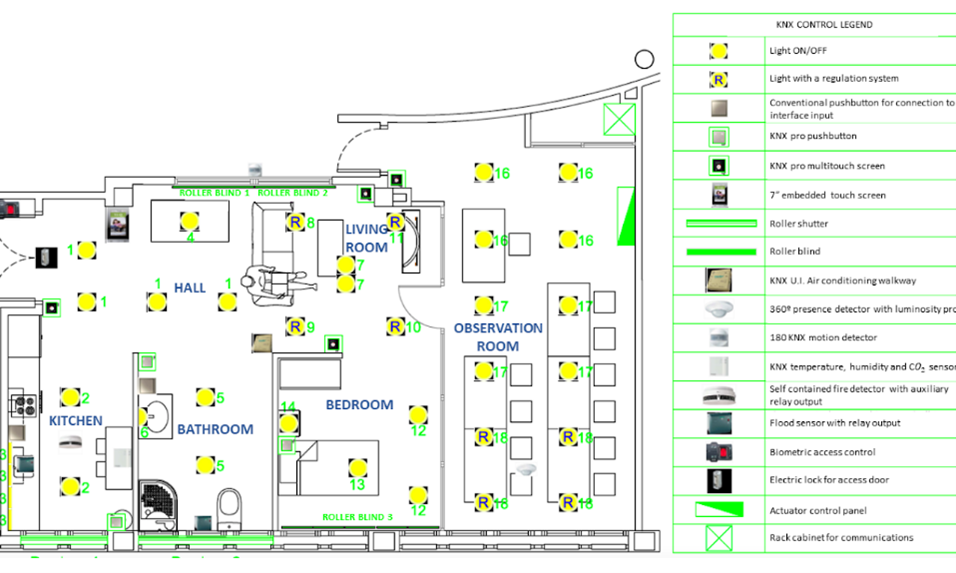
\includegraphics{imagenes/capitulo1/mapaSmarthome.png}
    \caption{Esquema de sensores y actuadores de la Smarthome}
    \label{fig:mapa_sensores}
\end{figure}

\subsection{Historia y desarrollo de KNX}

El origen de KNX es el resultado de la evolución de la domótica en las últimas décadas del siglo XX, pues se originó con la unión de tres estándares de los noventa: \textit{European Home Systems Protocol} (EHS), el \textit{European Installation Bus} (EIB) y el \textit{BatiBUS}, que pertenecían respectivamente a la \textit{European Home Systems Association} (EHSA), la \textit{European Installation Bus Association} (EIBA) y el \textit{BatiBUS Club International} (BCI).

El objetivo de esta unión era el desarrollo de un estándar común e internacional que facilitara la comunicación, gestión y compatibilidad de los dispositivos en el ámbito de la domótica. La estandarización de KNX junto con la aparición de las redes WiFi y los \textit{smartphones} proliferaron el desarrollo y el mercado de la domótica tanto a nivel industrial como doméstico durante los siguientes años \cite{intro_5}.

Gracias a esta estandarización, el control sobre la iluminación, calefacción y cualquier dispositivo KNX está es un mismo sistema, que con el paso de los años tiende a ser cada vez más automático. KNX y la domótica en sí ha ido evolucionando desde permitir controlar dispositivos a través de un panel de control o el móvil hasta no tener que controlarlo, ya que ahora mediante distintas condiciones, algoritmos e inteligencias artificiales, las decisiones y acciones se ejecutan solas.

Muchas veces, estas decisiones se toman en base a unos parámetros ideales. Por ejemplo, en este trabajo se usan parámetros atmosféricos como la temperatura o humedad, que el sistema trata de alcanzar y mantenerse. Muchas veces estos parámetros pueden ir directamente relacionados al consumo energético, de forma que se pueda controlar y limitar en todos los dispositivos, ya sea según el horario o avisando al usuario a través del móvil.

\subsection{Bases y funcionamiento de KNX}

Este protocolo parte de la idea de tener todos los dispositivos, que normalmente vamos a diferenciar entre sensores y actuadores, conectados a un “cable de comunicación” que permita intercambiar información entre ellos. Los sensores son dispositivos que detectan acciones y envían órdenes al bus en forma de telegramas. Los actuadores reciben estos telegramas y traducen las órdenes en acciones. De esta manera, un dispositivo sensor, por ejemplo, un sensor de presencia puede ordenarle a un dispositivo actuador como un relé que, siguiendo el ejemplo, encienda la luz.

\begin{figure}
    \centering
    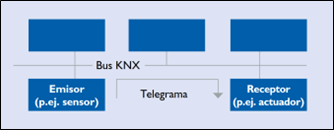
\includegraphics{imagenes/capitulo1/envioTelegrama.png}
    \caption{Envío de un telegrama por el bus KNX}
    \label{fig:envio_telegrama}
\end{figure}

Aunque la mayoría de los dispositivos se pueden englobar en sensores y actuadores, hay otros que no pueden agregarse a ninguna de estas categorías. Por ejemplo, hay muchos dispositivos con un objetivo visual, leyendo los valores de los sensores y actuadores pudiéndolo mostrar en pantallas a través de diferentes interfaces. También es común encontrar, sobre todo si la instalación es grande, un dispositivo que actúa como centro de control de toda la instalación KNX: los servidores web como SpaceLynk. Aunque más adelante hablaré algo más de este dispositivo, en resumen, permite no solo tener un control sobre todos los dispositivos conectados al bus, sino que tiene funcionalidades extras como el monitorio de la energía o el poder crear funciones lógicas que permitan codificar algoritmos que controlen los dispositivos según quiera el programador \cite{intro_6}.

Como ya he comentado, todos los dispositivos se encuentran conectados al mismo cable o bus. Esto significa que el acceso de estos al bus debe regularse y que la mayoría de los datos que se envían por el bus se utilizan para identificar a cada dispositivo que envía o reciba información. 
Este procesamiento no requiere de un dispositivo central que se encargue de dirigir los datos, sino que dicho trabajo se reparte entre todos los dispositivos del bus, ya que cada uno suele tener un microprocesador. Descentralizar la comunicación de dispositivos aporta gran autonomía al sistema, ya que, si fallara un dispositivo, no afectaría al resto de la instalación salvo a la que requiera específicamente de ese dispositivo. También aporta gran escalabilidad, aunque también depende en gran medida de la topología instalada, más adelante profundizaremos en ello.

\subsection{Medios de comunicación existentes}

\subsection{Topologías KNX más utilizadas}

\subsection{Listado de sensores utilizados en este trabajo}

% Los avances que se han producido en las tecnologías de redes son quizás los  más significativos en el mundo de hoy. Están ayudando a crear un mundo en el que las fronteras nacionales, las distancias geográficas y las limitaciones físicas se vuelven menos relevantes, presentando obstáculos cada vez menores.

% Esta revolución en las tecnologías de redes han permitido la aparición de servicios que hacen más fáciles las actividades habituales de las personas. La utilización del correo electrónico, la consulta de páginas web repletas de contenido, o el uso de foros para compartir información con otras personas, son ejemplos claros de estas nuevas tendencias. 

% Internet ha cambiado la forma en que ocurren nuestras interacciones sociales, comerciales, políticas y personales. La naturaleza inmediata de las comunicaciones por internet alienta la creación de comunidades globales que permiten la interacción social, independientemente de la ubicación o zona horaria.
	
% La creación de comunidades en línea para el intercambio de ideas e información tiene el potencial de aumentar las oportunidades de productividad en todo el mundo.
	
% La creación de la nube nos permite almacenar documentos e imágenes y acceder a ellos en cualquier lugar y en cualquier momento. Estemos en un tren, en un parque o en la cima de una montaña, podemos acceder sin problemas a nuestros datos y aplicaciones desde prácticamente cualquier dispositivo.

% Los avances en las tecnologías de redes han permitido, no sólo que las personas se conectan a Internet mediante innumerables aplicaciones y con distintos fines, sino también la aparición  de multitud de dispositivos conectados a Internet con el objetivo de dar y recibir datos para facilitar distintas acciones que las personas hacen en su vida cotidiana. Estos nuevos dispositivos son relojes, luces, neveras, hornos, etc. 

% En los últimos años, el número de dispositivos conectados a la red ha crecido de forma exponencial. En 2015 había poco más de 15 mil millones de dispositivos conectados a Internet\cite{thirtyfourth}, una media de 2 dispositivos por persona en el mundo. Actualmente existen 31 mil millones de dispositivos, y se espera que para el año 2025 haya un total de 75 mil millones de dispositivos conectados a la red, donde la mayoría serán objetos cotidianos de uso diario. La Figura \ref{fig:evolucion} muestra la evolución del número de dispositivos conectados. 

% %Aplicar efecto a las demás páginas
% \newpage
% \fancyhead{}
% \fancyfoot{}
% \renewcommand{\headrulewidth}{0.5pt}
% \fancyhead[LE,RO]{\textsl{\thepage}}
% \fancyhead[RE]{\textsl{\nouppercase{\leftmark}}}
% \fancyhead[LO]{\textsl{\nombreTFG}}

% \begin{figure}[h]
% 	\centering
% 	\includegraphics[width=.80\textwidth]{capitulos/capitulo1/evolucion.png} 
% 	\caption{Evolución del número de dispositivos conectados a Internet.}
% 	\label{fig:evolucion}
% \end{figure}

% Este mercado de nuevas cosas conectadas genera una cantidad de datos cada vez mayor. El volumen de datos que debe almacenarse y analizarse es inimaginable y sigue creciendo. La variedad de los datos seguirá expandiéndose a nuevas áreas que nunca antes estuvieron disponibles para el análisis. Las interacciones entre las personas que utilizan las plataformas de medios, la automatización de procesos, y el agregado de datos provenientes de fuentes diferentes crean lo que se conoce como Internet de las Cosas (IdC) ({\em Internet of Things} (IoT), en inglés). Esta transformación digital tiene un efecto profundo en tres elementos principales de nuestras vidas: lo empresarial, lo social y lo ambiental. Las interacciones en estas áreas crearán más datos para fomentar nuevas ideas, productos y soluciones. Esto producirá aún más datos nuevos, lo que resulta en un ciclo repetitivo de innovación exponencial que nos ayuda a tomar mejores decisiones y tener mejores ideas.

% En términos generales,  IoC ayuda a distintos sectores (Figura \ref{fig:areas}), como fabricación, servicios públicos, petróleo y gas, transporte, minería, y organizaciones públicas y privadas a aumentar la eficacia operativa. Las empresas y las ciudades implementan cada vez más soluciones de IoC. Sin embargo, éste rápido aumento en el crecimiento también presenta nuevos desafíos, a saber:

% \begin{itemize}
% 	\item Cómo integrar millones de dispositivos de diversos proveedores que utilizan aplicaciones personalizadas
% 	\item Cómo integrar dispositivos nuevas a la infraestructura de red existente
% 	\item Cómo proteger los dispositivos nuevos configurados con diversos niveles de seguridad
% \end{itemize}

% \begin{figure}[h]
% 	\centering
% 	\includegraphics[width=.70\textwidth]{capitulos/capitulo1/areas.png} 
% 	\caption{Sectores donde se aplica IdC.}
% 	\label{fig:areas}
% \end{figure}

% Esto de conectar los dispositivos a Internet para hacerlos más inteligentes no es algo de ahora, pues en 1982 se creó el primer dispositivo IdC. Una máquina de venta de refrescos que se conectaba a Internet para informar de cuando había refrescos fríos sin tener que ir físicamente donde estaba la máquina para comprobarlo \cite{thirtyfifth}.

% Internet de las cosas se encuentra a nuestro alrededor y se expande con rapidez. Apenas estamos comenzando a aprovechar sus beneficios. Constantemente se están desarrollando nuevas maneras de utilizar cosas conectadas. IdC ayuda a los individuos a conectar cosas para mejorar la calidad de vida.
% IdC también ayuda a las organizaciones e industrias a mejorar la administración de recursos para ser más eficientes. 

% En el ámbito industrial (IdCI), se ha incorporado conectando sensores inteligentes a Internet y usando esa información para tomar mejores decisiones comerciales. La mayor diferencia entre el IdC y el IdCI es que éste se ha diseñado para funcionar en espacios relativamente cerrados y con el objetivo de facilitar la comunicación con una empresa. Por ejemplo, una de las aplicaciones del IdCI es la detección de grandes concentraciones de polvo en entornos industriales para asegurar una mejor seguridad y salud de los trabajadores. La aparición de IdC en este ámbito ha significado una pequeña revolución industrial, cambiando los procesos productivos mediante la incorporación de estas nuevas tecnologías.

% En el ámbito de la agricultura ha permitido a los productores y agricultores reducir el desperdicio y mejorar la productividad, desde la cantidad de fertilizante utilizado hasta el combustible utilizado en la maquinaria agrícola. También se ha construido un sistema para monitorear el campo de cultivo con la ayuda de sensores (luz, humedad, temperatura y humedad del suelo) y la automatización del sistema de riego.

% En el ámbito sanitario, los dispositivos de IdC se han utilizado para el rastreo remoto de pacientes y sistemas de notificación de emergencias. Estos dispositivos pueden variar desde monitores de presión sanguínea y control de pulsaciones, hasta dispositivos capaces de seguir implantes especializados, como marcapasos, pulseras electrónicas o audífonos sofisticados. Algunos hospitales han comenzado a utilizar camas inteligentes que detectan cuándo están ocupadas y cuándo un paciente intenta levantarse. También puede ajustarse automáticamente para asegurar que el paciente tenga un soporte adecuado sin interacción del personal de enfermería. Pueden instalarse sensores especializados en espacios habitacionales para monitorear la salud y el estado de bienestar general de las personas mayores.

% Por último, pero no menos importante, en el ámbito del transporte se han usado para comunicaciones, controles y procesamiento de información a través de varios sistemas de transporte, ofreciendo soluciones a los múltiples desafíos que se presentan en toda la cadena logística. La aplicación de IdC se ha extendido a todos los aspectos de los sistemas de transporte (vehículos, infraestructura, conductores y usuarios). La interacción dinámica entre estos componentes de un sistema de transporte ha permitido la comunicación inter e intra vehicular, el control inteligente del tránsito, estacionamiento inteligente, cobro electrónico de peajes, logística y manejo de flota, control vehicular, seguridad y asistencia en rutas.  En logística y manejo de flota, por ejemplo, la plataforma de IdC puede hacer seguimiento en todo momento de la ubicación y las condiciones de la carga y los activos mediante sensores inalámbricos que envían alertas en caso de eventualidades, tales como demoras, daños, o robos entre otras.

% \section{Smarthome: Tecnología inteligente para el hogar}

% Dentro del campo de aplicación del Internet de las Cosas, se encuentran las {\bf Casas Inteligentes} ({\em Smart Homes} en inglés). Estas viviendas están compuestas por una gran variedad de sensores y actuadores capaces de realizar ciertas acciones de forma automatizada sin la intervención del usuario con el objetivo de mejorar la experiencia de éste.

% La tecnología inteligente para el hogar ha sido descrita desde distintas perspectivas \cite{first}. Desde un punto de vista tecnológico,  puede definirse como “una inteligencia omnipresente y transparente en un entorno vigilado que soporta las actividades e interacciones de los usuarios”. La visión principal de la inteligencia en el hogar presenta al usuario rodeado de interfaces inteligentes e intuitivas, integradas en los objetos cotidianos de su entorno de forma transparente. Estas interfaces poseen capacidad para reconocer la presencia de diferentes usuarios, y modificar su comportamiento en función de la identidad de dicho usuario, sus necesidades y las características del contexto o entorno donde se encuentren. Especial atención merecen aspectos como la facilidad de uso, el soporte eficiente de los servicios y la posibilidad de mantener interacciones naturales con las personas. Su gran relevancia reside en los importantes cambios que, a no muy largo plazo, implicarán sus resultados en la vida diaria de las personas \cite{second, third}. 

% La inteligencia en el hogar consiste en la creación de espacios donde los usuarios interaccionen de forma natural y sin esfuerzo con los diferentes sistemas, gracias a que las tecnologías de computación y comunicación se convierten, en estos entornos, en invisibles para el usuario, al estar siempre presentes e integradas en los objetos cotidianos del mismo \cite{fourth, fifth}. De esta forma, es la propia tecnología la que se adapta a los individuos y a su contexto, actuando de forma autónoma, y facilitándoles la realización de sus tareas diarias y la comunicación entre ellos y con el entorno. 

% Esta visión ha despertado un creciente interés por utilizar las tecnologías de la computación en la construcción de sistemas que soporten las actividades de la vida diaria de forma más eficiente \cite{sixth, seventh, eighth}. En este contexto, uno de los elementos más importantes de una vivienda es el frigorífico, el cual nos permite obtener alimentos frescos para cocinar y alimentarnos. 
 
% En este Trabajo Fin de Grado se van a implantar diferentes sensores en el frigorífico ubicado en la SmartHome de la Universidad de Almería (SH-UAL) con el objetivo de dotarlo de inteligencia. A partir de los datos generados por los dispositivos, se podrá, entre otras: (i) automatizar la lista de la compra; (ii) dar consejos para una dieta más equilibrada; o incluso (iii) establecer rutinas alimenticias para personas con dependencia. 

% %%Explicacion de la smarthome
% La SH-UAL está construida en el laboratorio 2.29 del CITE III. En el siguiente enlace [\url{https://youtu.be/6jcUtaQR-lc}] podemos ver un vídeo de las distintas estancias que la componen. Como puede verse, esta dispone de dos diferentes áreas. Primeramente tiene un aula/laboratorio con ordenadores, desde los que se puede controlar toda la vivienda. Esta parte está enfocada a prácticas docentes. La segunda parte se corresponde con la vivienda en sí, la cual está formada por:

% \begin{multicols}{2}
%     \begin{itemize}
%     	\item Distribuidor.
%     	\item Zona de trabajo.
%     	\item Salón.
%     	\item Cocina.
%     	\item Baño.
%     	\item Dormitorio.
%     \end{itemize}
% \end{multicols}

% La vivienda está equipada con un conjunto de sensores y actuadores para dotarla de inteligencia. La Figura \ref{fig:smarthome1} muestra una vista de la casa, dónde se aprecia el salón, dormitorio y parte del baño. La Figura \ref{fig:smarthome2} muestra otra perspectiva de la casa. En ella se puede visualizar parte del baño, la cocina y la entrada a la vivienda.

% En la cocina de la SH-UAL se encuentra un frigorífico modelo LG-GSX961NSAZ, la Figura \ref{fig:fridge} muestra la vista del mismo. Este frigorífico será el objeto de estudio de este TFG. En concreto se le instalarán una serie de sensores y se le incluirán mecanismos de inteligencia artificial para la toma de decisiones. Así, a partir de los datos generados por los sensores, se podrá automatizar la lista de la compra, saber que productos ha consumido un usuario, o el número exacto de productos en el interior del mismo. 

% \begin{figure}[h]
% 	\centering
% 	\includegraphics[width=.70\textwidth]{capitulos/capitulo1/smarthome1.png} 
% 	\caption{Casa inteligente de la Universidad de Almería}
% 	\label{fig:smarthome1}
% \end{figure}

% \begin{figure}[h]
% 	\centering
% 	\includegraphics[width=.70\textwidth]{capitulos/capitulo1/smarthome2.png} 
% 	\caption{Casa inteligente de la Universidad de Almería}
% 	\label{fig:smarthome2}
% \end{figure}

% \begin{figure}[h]
% 	\centering
% 	\includegraphics[width=.25\textwidth]{capitulos/capitulo1/fridge.png} 
% 	\caption{Frigorífico LG-GSX961NSAZ}
% 	\label{fig:fridge}
% \end{figure}

% \newpage
% \section{Herramientas usadas}

% En esta sección se va a realizar una descripción de las herramientas que se han usado para desarrollar el trabajo. Para ordenar las herramientas, se han dividido en diferentes categorías.

% \subsection{Lenguajes de programación}

% En esta categoría se describen los lenguajes de programación que se han usado para realizar el proyecto.

% \subsubsection{JavaScript}

% \begin{wrapfigure}{r}{2.1cm}
%   \scalebox{0.04}{
%     \includegraphics{capitulos/capitulo1/js.png}
%   }
% \end{wrapfigure}

% JavaScript \cite{eleventh} es un lenguaje de programación que antes se utilizaba principalmente para crear páginas web dinámicas. Hoy en día, se puede utilizar también para crear el lado del servidor.

% Técnicamente, JavaScript es un lenguaje de programación interpretado, por lo que no es necesario compilar los programas para ejecutarlos. Esto permite que se puedan probar directamente en cualquier navegador, sin necesidad de procesos intermedios.

% Este lenguaje se utiliza para crear framework como NodeJS, ReactJS o Express, por lo que ha sido el lenguaje principal en el desarrollo de este trabajo. Se ha decidido usar este lenguaje ya que es un lenguaje bastante optimizado para el desarrollo de sistemas web, el cual se puede utilizar para el desarrollo de la parte del cliente y del servidor.

% \subsubsection{HTML}

% \begin{wrapfigure}{r}{1.7cm}
%   \scalebox{0.2}{
%     \includegraphics{capitulos/capitulo1/html.png}
%   }
% \end{wrapfigure}

% HTML [HyperText Markup Language (Lenguaje de marcas de hipertexto)] \cite{twelfth} es un lenguaje basado en etiquetas que su uso principal es la creación de páginas web. Este lenguaje es soportado por todos los navegadores actuales. 

% En este proyecto se utilizará para crear la interfaz del usuario en complementación con ReactJS. Se utilizará este lenguaje para crear la interfaz porque es un lenguaje utilizado desde hace mucho tiempo, por lo que hay mucha cantidad de información y soporte a través de Internet.

% \subsubsection{CSS}

% \begin{wrapfigure}{r}{1.7cm}
%   \scalebox{0.2}{
%     \includegraphics{capitulos/capitulo1/css.jpg}
%   }
% \end{wrapfigure}

% CSS [Cascading Style Sheets (Hojas de estilo en cascada)]\cite{thirteenth}  es un lenguaje que es usado para complementar el HTML y darles diseño a las páginas web y poder personalizarlas al gusto del usuario. Actualmente es el lenguaje más usado para personalizar páginas web.

% En nuestro proyecto se va a utilizar un framework llamado BootStrap 4.0, que incluye muchas clases CSS predefinidas que se pueden aplicar a las etiquetas HTML y así personalizarlas sin tener que crear el código CSS desde cero.

% \subsubsection{\LaTeX}

% \begin{wrapfigure}{r}{2cm}
%   \scalebox{0.2}{
%     \includegraphics{capitulos/capitulo1/latex.png}
%   }
% \end{wrapfigure}

% \LaTeX\cite{fourteenth} es un lenguaje de tipografía, con el que se puede crear documentos de bastante calidad. Este lenguaje está formado por órdenes construidas a partir de comandos \TeX, por lo que es un lenguaje de bajo nivel.

% Dado que mucha gente lo utiliza cuando necesita redactar un documento importante, como una investigación o una memoria de un proyecto, se ha decidido utilizar este lenguaje para redactar la memoria de este proyecto.

% \subsection{Comunicación}
% A continuación, se muestran las diferentes formas de comunicación que se han realizado entre el alumno y los tutores a lo largo del desarrollo del trabajo.

% \subsubsection{Correo electrónico}
% Cuando se ha tenido que hacer una comunicación entre el alumno y los tutores a distancia, se ha usado el correo electrónico. De esta manera, todo lo hablado se queda ordenado cronológicamente y accesible en cualquier momento. También se ha utilizado para concertar reuniones, o enviar enlaces a vídeos que el alumno ha grabado para mostrar el progreso del trabajo.

% \subsubsection{Vídeos}
% El alumno ha utilizado vídeos que ha adjuntado en algunos correos electrónicos para mostrarle a los tutores el progreso del proyecto sin necesidad de tener que estar físicamente presenciales. Estos vídeos son vistos por los tutores y proponen cambios o sugerencias para que el proyecto quede lo mejor posible entre ambos.

% \subsubsection{Reuniones}
% Las reuniones presenciales han sido necesarias al inicio del proyecto para definirlo, y durante éste para diferentes dudas. Es la mejor forma ya que es presencial y obtienes una respuesta inmediata.


% \subsection{Desarrollo}
% En esta categoría se va a explicar los diferentes entornos que se han utilizado para el desarrollo del proyecto.

% \subsubsection{Visual Studio Code}

% \begin{wrapfigure}{r}{2cm}
%   \scalebox{0.04}{
%     \includegraphics{capitulos/capitulo1/vscode.png}
%   }
% \end{wrapfigure}

% Visual Studio Code\cite{fifteenth} es un IDE (aplicación informática que proporciona servicios integrales para facilitarle al desarrollador o programador el desarrollo de software) desarrollado por Microsoft para Windows, Linux y macOS. Su principal característica es que incluye soporte para la depuración de muchos códigos, como PHP, JavaScript, etc. También permite instalar complementos de todos los lenguajes y adaptándose a ellos.

% Este IDE va a ser utilizado para hacer toda la codificación del proyecto, dado que funciona muy bien para programar con JavaScript e incluye numerosos plugins (aplicación que se relaciona con otra para agregarle una función nueva y generalmente muy específica) que complementan al IDE y permiten personalizarlo al máximo para dejarlo al gusto del usuario. También hay que destacar que el alumno ha usado anteriormente este IDE y se siente muy familiarizado con él, que es otro punto positivo a tener en cuenta.

% \subsubsection{OneDrive}

% \begin{wrapfigure}{r}{2cm}
%   \scalebox{0.08}{
%     \includegraphics{capitulos/capitulo1/onedrive.png}
%   }
% \end{wrapfigure}

% OneDrive\cite{sixteenth} es un servicio de alojamiento de archivos en el que se han guardado los archivos necesarios para que el sistema funcionara conforme se iba creando. Cada vez que se crea un cambio, éste se queda registrado y se puede volver a versiones anteriores si es necesario. También los cambios se suben a la nube para que estén seguros en caso de perdida de los archivos locales.

% Al estar en la nube, eran fácilmente compartibles entre otras personas, como los tutores, que han revisado periódicamente el progreso del trabajo para asegurarse que todo estaba correctamente realizado.

% Se ha usado esta opción porque el alumno tiene acceso a un alojamiento gratuito con la cuenta de la Universidad. Además, tiene configurado todos sus dispositivos con esta aplicación y, guardando el proyecto aquí, se guarda en todos los dispositivos del alumno automáticamente.

% \subsubsection{Insomnia}

% \begin{wrapfigure}{r}{1.8cm}
%   \scalebox{0.11}{
%     \includegraphics{capitulos/capitulo1/insomnia.jpg}
%   }
% \end{wrapfigure}

% Insomnia\cite{seventeenth} se trata de una herramienta desarrollada para realizar peticiones GET, POST, PUT y DELETE a cualquier sistema. De esta manera, se puede testear opciones del servidor para asegurarnos de que funciona correctamente antes de tener que realizar la parte del cliente.

% Se ha utilizado esta aplicación porque es bastante completa y es la que recomiendan en los diferentes sitios donde el alumno ha navegado para aprender acerca de stack MERN.

% \subsubsection{Tinkercad}

% \begin{wrapfigure}{r}{1.7cm}
%   \scalebox{0.16}{
%     \includegraphics{capitulos/capitulo1/thinkercad.png}
%   }
% \end{wrapfigure}

% Tinkercad\cite{eighteenth} es una página web que ofrece un servicio para hacer modelos 3D de forma gratuita. Una vez registrado, tienes acceso a poder crear diferentes proyectos con diferentes modelos. Puedes subir tus propios modelos 3D y modificarlos, o crearlos directamente desde cero con objetos sencillos que ofrece la página, y con la posibilidad de unirlos o separarlos.

% El alumno utiliza esta página para crear los modelos 3D necesarios para imprimir diferentes piezas que se usan para implementar correctamente los sensores en el frigorífico.

% Esta página es una de las más famosas a la hora de realizar modelos 3D, además de ser gratuita, por lo que se ha escogido esta página por estas razones.

% \subsubsection{Ultimaker Cura}

% \begin{wrapfigure}{r}{1.8cm}
%   \scalebox{0.18}{
%     \includegraphics{capitulos/capitulo1/cura.png}
%   }
% \end{wrapfigure}

% Ultimaker Cura\cite{nineteenth} es un software que nos permite cargar un modelo 3D y prepararlo para imprimirlo en una impresora 3D. Una vez que se especifica el material y la impresora a usar, se carga el modelo y se coloca dentro de la superficie de impresión (se puede mover, redimensionar, girar y demás opciones dentro del programa), se puede pasar a laminar el modelo y ponerle soportes si es necesario, y con todo esto está listo para imprimir.

% Se ha elegido este software porque es gratuito y después de hacer pruebas con otros software, es el que mejor crea los soportes para el objeto, por lo que el alumno ha elegido este software por esas razones.

% \subsection{Documentación}
% En esta sección se muestran las herramientas que se han utilizado para realizar la documentación del proyecto que se ha realizado.

% \subsubsection{OverLeaf}

% \begin{wrapfigure}{r}{1.8cm}
%   \scalebox{0.07}{
%     \includegraphics{capitulos/capitulo1/overleaf.jpg}
%   }
% \end{wrapfigure}

% Es un editor de código \LaTeX, que cuenta con algunas ventajas que otros no cuentan, como por ejemplo que es gratuito y online. De esta manera, todo se queda alojado en la nube y se puede acceder desde cualquier todo dispositivo con acceso a Internet. También te avisa de errores de sintaxis para que puedas arreglarlo, y va generando el resultado visual del código conforme escribes, sabiendo en cualquier momento como está quedando el texto una vez terminado.

% Se ha usado esta herramienta por todas las ventajas comentadas anteriormente, además de que es una de las plataformas mas usadas actualmente para la edición de \LaTeX.

% \subsubsection{Google Drive Docs}

% \begin{wrapfigure}{r}{1.4cm}
%   \scalebox{0.09}{
%     \includegraphics{capitulos/capitulo1/gdc.png}
%   }
% \end{wrapfigure}

% Google Drive Docs\cite{twentieth} es una herramienta que permite editar documentos de texto, parecido a Word de Microsoft, con la diferencia de que esta es online y se aloja en la nube, con las ventajas que esto conlleva, como por ejemplo el poder trabajar diferentes personas sobre en mismo documento, o el autoguardado cada cambio que se hace.

% Se ha usado esta herramienta para realizar un escrito previo del proyecto y compartirlo con los tutores para que le hagan un seguimiento y sugerir cambios. También dispone de un historial de cambios, pudiendo volver a una versión anterior si en algún momento es necesario.

% \subsubsection{GreenShot}

% \begin{wrapfigure}{r}{1.9cm}
%   \scalebox{0.04}{
%     \includegraphics{capitulos/capitulo1/greenshot.png}
%   }
% \end{wrapfigure}

% GreenShot\cite{twentyfirst} realiza capturas de pantalla de una forma muy cómoda y rápida. Permite realizarlas solo de un área de la pantalla en concreto y una vez hecha, permite guardarla en una ubicación en específico, o dejarla copiada en el portapapeles para pegarla directamente. Te permite también editar la captura antes de guardarla, por lo que es útil por si quieres remarcar algo en la captura.

% Se ha elegido este software para las diferentes capturas de pantallas necesarias a lo largo de este proyecto, como capturas de pantalla para recoger las diferentes vistas de la interfaz acabada, o para adjuntar alguna captura con información a los tutores para alguna posible duda a lo largo de la realización del proyecto.

% \subsubsection{GanttProject}

% \begin{wrapfigure}{r}{1.8cm}
%   \scalebox{0.18}{
%     \includegraphics{capitulos/capitulo1/gantt.png}
%   }
% \end{wrapfigure}

% El diagrama de Gantt es una de las herramientas más usadas para la gestión de proyectos. Con este diagrama se realiza la planificación de las tareas a lo largo del tiempo con el objetivo de realizar el proyecto de forma correcta. Con esta herramienta se puede ver de una manera general el tiempo que se ha invertido en cada una de las tareas, así como el orden en el que se han realizado.

% El software GranttProject se trata de un software de código abierto que permite la realización de estimaciones en forma de diagramas de Gantt. Se ha decidido hacer uso de esta herramienta por su facilidad de uso.

% \subsubsection{Visual Paradigm Online}

% \begin{wrapfigure}{r}{1.8cm}
%   \scalebox{0.15}{
%     \includegraphics{capitulos/capitulo1/visualparadigm.png}
%   }
% \end{wrapfigure}

% Visual Paradign Online es una página web que permite muchos tipos de diagramas de forma sencilla y gratuita. También es online, con todas las ventajas que añade esto. Uno de estos diagramas que permite realizar, es el diagrama de actividades, y es el que se usa para explicar como funciona el sistema en algunas situaciones.

% Se ha usado esta herramienta porque es gratuita y permite hacer los diagramas necesarios para explicar los procesos necesarios del sistema, por lo que cumple todos los requisitos necesarios.

% \subsection{Stack MERN}
% En esta sección se va a explicar las tecnologías usadas para la realización de este proyecto y para su correcto funcionamiento.

% El stack MERN\cite{nineth} es un conjunto de tecnologías que están relacionadas entre sí y que tienen como objetivo la creación de un servicio web de una forma eficiente y sencilla para el usuario. Con todo este conjunto de tecnologías se puede llegar a crear tanto el back-end (parte de una web que se encarga de que toda la parte lógica de una página web funcione) como el front-end (parte de una web que conecta al back-end e interactúa con los usuarios que la visitan a través de una interfaz) del sistema.

% El crear un conjunto de tecnologías para la creación de sistemas no es nuevo, anterior a éste, existía LAMP (Linux, Apache, MySQL y PHP) o MEAN (MongoDB, Express, AngularJS, NodeJS), pero actualmente el más usado es el que se está presentando (MongoDB, Express, React, NodeJS).

% Todas estas tecnologías se usan para el back-end, excepto React, que es una librería del front-end que se utilizará para crear y gestionar toda la interfaz. 

% Otra característica de MERN es que el lenguaje de programación en todas estas tecnologías es el mismo. Se utiliza JavaScript para programar tanto el back-end como el front-end.

% \subsubsection{MongoDB}

% \begin{wrapfigure}{r}{2.5cm}
%   \scalebox{0.04}{
%     \includegraphics{capitulos/capitulo1/mongo.png}
%   }
% \end{wrapfigure}

% MongoDB\cite{twentysecond} se trata de la base de datos que se usa en la estructura MERN. Esta base de datos fue creada en 2007 y es una base de datos no relacional, es decir, no está formada como las bases de datos SQL con tablas y columnas, sino por colecciones y documentos. Así, estos documentos están formados en el lenguaje JSON, que permite un fácil manejo de estos. Una de las características de éste, es que no tiene un esquema predefinido, por lo que permite una gran flexibilidad en la información que almacena.

% Se ha usado esta base de datos porque en este sistema se va a almacenar mucha información de los sensores, y al ser una base de datos no estructurada que permite la indexación, realiza las operaciones con mayor velocidad que si se utilizara una base de datos relacionada.

% \subsubsection{Mongoose}

% \begin{wrapfigure}{r}{2.8cm}
%   \scalebox{0.4}{
%     \includegraphics{capitulos/capitulo1/mongoose.jpg}
%   }
% \end{wrapfigure}

% Mongoose\cite{twentyrhird} es una biblioteca que nos permite hacer varias opciones con la base de datos de MongoDB, como conectarnos a la base de datos o crear esquemas, por ejemplo. En este proyecto se ha utilizado por ejemplo para hacer una conexión entre la base de datos y la parte del back-end que se encarga de hacer modificaciones sobre esta.

% Se ha utilizado este sistema para crear la conexión y los esquemas de la base de datos ya que es la utilizada en todos los tutoriales visualizados por el alumno que ha realizado el proyecto.

% \subsubsection{ExpressJS}

% \begin{wrapfigure}{r}{2.8cm}
%   \scalebox{0.1}{
%     \includegraphics{capitulos/capitulo1/express.png}
%   }
% \end{wrapfigure}

% ExpressJS\cite{twentyfourth} se trata de un framework que permite simplificar las tareas de escribir código para el servidor que maneja el sistema. Dado que el servidor contiene código JavaScript ejecutado por NodeJS, Express proporciona las herramientas necesarias para garantizar el correcto funcionamiento del servidor de NodeJS. Express proporciona un framework web para usar NodeJS como servidor de una aplicación web. 

% \subsubsection{NodeJS}

% \begin{wrapfigure}{r}{2.8cm}
%   \scalebox{0.22}{
%     \includegraphics{capitulos/capitulo1/node.png}
%   }
% \end{wrapfigure}

% NodeJS\cite{twentyfifth} se trata del entorno que permite la ejecución de código JavaScript independientemente del navegador, por lo que se pueden ejecutar scripts de JavaScript en el terminal local de un PC usando NodeJS. Este entorno permite la instalación de librerías para incluir funcionalidad a los scripts de JavaScript que se ejecuten. De todas formas, se pueden realizar tareas de programación que tradicionalmente han sido realizadas en lenguajes como Python o C, usando JavaScript. Actualmente está muy de moda para el desarrollo de servicios web, permitiendo realizar las funciones de back-end en JavaScript, lenguajes que nunca habían sido usados fuera del entorno del front-end.

% Se ha decidido usar NodeJS para la ejecución de scripts en el controlador de IdC que se ha incluido en el proyecto, además de para el desarrollo del sistema.

% \subsubsection{Axios}

% \begin{wrapfigure}{r}{2.0cm}
%   \scalebox{0.04}{
%     \includegraphics{capitulos/capitulo1/axios.png}
%   }
% \end{wrapfigure}

% Axios\cite{twentysixth} es una librería de JavaScript que permite enviar peticiones GET, POST, PUT y DELETE desde cualquier archivo JavaScript hacia una dirección que se especifique. Esto nos valdrá para enviar peticiones al back-end desde el front-end o desde los controladores para hacer acciones en éste, como la creación, modificación o eliminación de algún objeto de la base de datos.

% Se ha usado esta librería porque era necesario un método para enviar peticiones al back-end desde fuera para hacer ciertas acciones, y el alumno investigando ha llegado a la conclusión de que la más usada era esta.

% \subsubsection{React}

% \begin{wrapfigure}{r}{2.8cm}
%   \scalebox{0.04}{
%     \includegraphics{capitulos/capitulo1/react.png}
%   }
% \end{wrapfigure}

% React\cite{twentyseventh} es una librería de JavaScript creada por Facebook. Esta librería permite la creación de componentes, elementos que gestionan su estado y tienen funcionalidad propia, pudiendo interactuar con otros componentes padres o hijos con los que estén relacionados. Además, React maneja vistas declarativas, por lo que el usuario no tiene que preocuparse de los efectos que se producen cuando una vista cambia de estado debido a cambios en los datos de esta. En definitiva, incluye funciones que normalmente están incluidas en jQuery, pero de forma nativa.

% Se ha usado React con el objetivo de lograr un alto grado de separación de funcionalidad entre las vistas, además de proporcionar código de jQuery de forma nativa, sin tener que preocuparse por la visualización de los elementos y el contenido dinámico de la interfaz.

% \subsubsection{Comunicación entre Arduinos y MondogDB}

% Adicionalmente al sistema MERN, se ha utilizado un archivo por controlador que importa la librería axios para hacer conexión con el back-end y otra librería que se mostrará posteriormente para hacer conexión con una controladora Arduino\cite{twentyeighth}. De esta manera, este archivo hace de intermediario entre el controlador (sensores) y el back-end y es el encargado de recibir los datos de los sensores y de producir acciones en el back-end dependiendo de lo que llegue. 

% Este archivo también está escrito en JavaScript y se necesita uno por cada Arduino utilizada en el proyecto. Cada Arduino se identifica con su IP privada, y envían sus datos a la misma IP (back-end) a través de un puerto diferente para diferenciarlas.